%Tudo que começa com '%' é comentário e é ignorado pelo compilador

%Gerando arquivo em latex:
%latex arquivo.tex (em dvi)
%pdflatex arquivo (em pdf)
%dvipdfm arquivo
%s2pdf arquivo

% Alguns modos de usar o latex:
% Windows – Miktex com Led
% Linux – texlive com kile

\documentclass[12pt]{report} %aqui fala o tipo de documento e o tamanho da fonte. Opções: tamanho do texto (10pt, 12pt, 14pt), formato do papel (a4paper, a5paper, b5paper, letterpaper, legalpaper, executivepaper), o número de colunas (onecolumn, twocolumn), entre outras opções.
%Por exemplo, [12pt,a4,twocolumn].
%classe: article, report, letter, book ou slides. Instalar abnt para quem está pensando no tf
\usepackage[brazilian]{babel} %hifenização em português do brasil
\usepackage[T1]{fontenc} % caracteres com acentos são considerados um bloco só
\usepackage[utf8]{inputenc} % Corrigie os acentos em Português
\usepackage{ae} %arruma a fonte quando usa o pacote fontenc
%\usepackage[pdftex]{graphicx}%Para inserir figuras
\usepackage{vhistory}
\usepackage{graphicx}

\begin{document}
\title{ICTP - Aceleradores 2015}
\author{Vitor Vasconcelos Araújo Silva\\ vitors@cdtn.br}
\date{\today}

\maketitle %cria o título

%\def \negritovi {\textbf} %Criando comandos

%\tableofcontents %índice
%\pagebreak % Quebra de página
%\listoffigures %indice de figuras
%\listoftables %indice de tabelas
%\pagebreak % Quebra de página

\begin{abstract}
  Este documento armazena - sem maior organização - as anotações feitas
  no curso sobre GPUs no ICTP em 2015.
\end{abstract}

%\begin{versionhistory}
%	\vhEntry{0.0}{30/11/2018}{Vitor}{Documento criado}
%	\vhEntry{1.1}{23.01.04}{DP|JPW}{correction}
%    \vhEntry{1.2}{03.02.04}{DP|JPW}{revised after review}
%\end{versionhistory}

\chapter*{Anotações}
\section*{\date{25/05/2015}: 1o. dia - Arquiteturas}

\begin{itemize}
	\item[V4]-
	\item[V5]- Hyper-threading -> melhora a utilização geral mas não do programa individual. 2/3 ou 3/4 do cores é melho do que todos no nodo. Weird reason que ele não explicou (para essa arquitetura).
	\item[V6]- Multi-core -> precisa de aplicação paralela para ser útil.
	\item[V7]- Aceleradores -> Não têm OS, diminui o overhead.
\end{itemize}

Atenção à hierarquia dos dados.

\subsection*{Ivan Girotto: basics das aceleradoras}

Problemas paralelizáveis: MC(Serpent) em GPUs?

Forma geral de se implementar em GPUs:
\begin{itemize}
	\item[1]: Copiar dados da CPU para GPU (bottleneck da velocidade)
	\item[2]: Launch kernel(instrumenar a GPU, colocar a função na GPU)
	\item[3]: Executar a função na GPU
	\item[4]: Copiar do resultado de volta da GPU -> CPU
\end{itemize}

Intel MIMD: funciona como um cluster. A interface varia: mais de uma forma de se comunicar com a planca (Intel XEON Phi).

CUDA é a aiblioteca de programação. Nada a ver com a capacidade de processamento. 
Importante: o sumário dele dá um bom resumo, pegar a apresentação.

\subsection*{Basic laboratory}

Utilizado o Linux Mint.

ISSA: id004919

passwd: xxxxxxxx

scratch/<user> -> todos os nós podem ler ali. I/O especial e mais apropriado. Lugar para coloca arquivos de entrada e saída.

Scheduler: TORQUE

\texttt{qstat -q}

\texttt{qstat -u \$USER}

\texttt{qstat -Q}: Lista de filas: wide, GPU, etc... Nós estamos na queue reserved2


MODULES: permite que eu escolha os módulos que vou rodar. Ex.: diferentes versões de bibliotecas, compiladores, etc.

comando: \texttt{module} (o mesmo da instalação do OpenMPI no Linux)

texttt{module local intel/14.0}

which icc -> me mostra o icc no path

module list -> mostra os módulos que carreguei

login nodes: geralmente só para logar, nunca para executar.

\texttt{qsub my-script1.sh} -> mostra se meu job foi enviado.

\texttt{nvidia-smi} -> é o gerenciador do sistema Nvidia.

O compilador cu avisa pro nvcc que o código tem C e CUDA. Opção do compilador:

\texttt{-arch =sm\_35}: specific name of clan of Nvidia GPU para o CUDA. 

\texttt{-pg}: debug para código CPU

\texttt{-G}: debug para código GPU

\texttt{--ptxas-options = -u}: mostra os recursos GPU sendo gastos

\textbf{OpenACC} é um padrão de programação. Nível acima do CUDA, aparentemente.
(adição 2018) Este padrão usa decoração de código, como no OpenMP, para adicionar 
paralelismo ao código que se pretende levar para a GPU. Não escala bem: programação 
para GPU tem que ser pensada para GPU (\textit{Introduction do GPU Architecture and Programming Models | Tim Warburton, Virginia Tech, ATPESC 2018})


\subsection*{Lab2/dia1}

4 exemplos diferentes.

\texttt{qdel <process-id>}: deleta o processo da fila

Tempo de compilação: ~7 segundos. 128, 1024, 4096, 8192, 16384.

Candidato a usar em GPU: Seções de choque (Por que eu anotei isso? Foi só uma ideia perdida, acho).

"Algumas vezes a força bruta é a resposta correta.". Em algums problemas, a leitura 
de tabelas prontas em disco é mais "cara" do que usar a GPU para computá-las.

Para logar no sissa: meu id004919
frontend1.hpc.sissa.it

\date{26/05/2015}, \date{28/05/2015} e \date{03/06/2015}: dias no laboratório pequeno.

\texttt{qstat -u \$user -n}  -> mostra o que está alocado só para mim.

Hoje: pensar em paralelo, programar em paralelo.

CUDA C -> Curiosidade: ver a origem do CUDA.

Accelerator -> a complete separated device.

GPU \textit{threads}: light weigth.

GPU é eficiente a partir de milhares de \textit{threads}.

CPU e sua memória: host.

GPU e sua memória: device.

\texttt{--host--, --global--, --device--}: parâmetros que definem onde será executado o código (particionamento).

\texttt{--shared--, --device--, --constant--}: data partitioning.

\texttt{--global-- e --device--} são executados por múltiplas \textit{threads}.

É função do programador saber que elas são executadas por múltiplas \textit{threads}.

?: como fica a memória? Cada \textit{thread} tem a sua, certo?

Exemplo: (Acho que aqui já tá falando do CUDA em si ou OpenACC)

\begin{verbatim}
int add(int a, int b) : add(a, b)
					   add<<<x, y>>>(a, b)
\end{verbatim}
Acima, x e y são o número de \textit{threads}.

global functions são todas 'void'. Se quiser passar algum parâmetro tem que 
ser via argumentos (tal qual o OpenCL, que aprendi depois).

Função \texttt{add}: (os argumentos são ponteiros)
\begin{verbatim}
--global-- void add(int *a, int *b, int *c) {
	*c = *a + *b;
	}
\end{verbatim}

\texttt{--global--} significa: \texttt{add} será executada no \textit{device} e 
\texttt{add} será chamada pelo \textit{host}.

Copiar memória:
\begin{verbatim}
cudaMalloc(&p, size);
cudaFree(p);
cudaMemcpy(t, s, size, direction);
\end{verbatim}

As referências são passadas dentro da função:

\begin{verbatim}
swap(&a, &b)

swap(int *a, int *b) {
	
	int *tmp = *(a);
	*(a) = *(b);
	b = tmp;
}

int *p;
p = malloc(sizeof(int)*tamanho); // tamanho do vetor

            ----CUDA---
            
void cudaMalloc(&p, tam); 
// o CUDA não retorna valor, tam é o tamanho do inteiro
\end{verbatim}

Cuda error checking \texttt{cudaError\_t cudaMalloc(void **devPtr, size\_t size)}

\begin{verbatim}
cudaError_t error;
error = cudaGetLastError();
if(error != cudaSuccess)
{
	printf("Erro no kernel: %s\n", cudaGetErrorString(error));
}
\end{verbatim}

O que falamos aqui: cópias assíncronas. Garantia de que, na próxima linha tenho tudo o que copiei. Isso quando é uma chamada depois da outra do CUDA. Se chamo 
código C depois, não tenho garantia de sincronia.

Usando block e \textit{threads} no CUDA:

\begin{verbatim}
add <<<1,1>>>(...)
add <<<n,nt>>>(...)
\end{verbatim}

\texttt{add} é executada n vezes em paralelo. Cada chamada ao \texttt{add} é um "bloco". Não existe loop. \texttt{n} é o número de blocos e \texttt{nt} 
é o número de \textit{threads} no bloco.

\texttt{blockIdx.x}: índice do bloco em que a \textit{thread} será executada.
\texttt{threadIdx.x}: índice da \textit{thread} a ser executada.
\texttt{blockDim.x}: dimensão do bloco (tamanho do bloco).

(Basicamente, o kernel do CUDA elimina os loops - pensar sempre em loops 
aninhados nos quais os índices acima são usados para referenciar de 
forma aninhada - que são definidos, na prática, na chamada do kernel 
(\texttt{<<< >>>})).

\texttt{.x, .y, .z}. As coisas existem em 3D (3D de blocos). Definir 
as dimensões:

\begin{verbatim}
dim3 gridDim;
dim3 blockDim;
dim3 blockIdx;
dim3 threadIdx;
\end{verbatim}

Exemplo:
\begin{verbatim}
dim3 bb;
bb.x = 100;
bb.y = 50;

add <<< bb, 1 >>> (a, b, c)
\end{verbatim}

Esse bloco vira \texttt{gridDim}, ver a diferença.

\section*{\date{26/05/2015}: Laboratório: tarde}

3 versões: paralelizar com blocks, \textit{threads} e blocks/\textit{threads}.

load módulo de CUDA, nvcc.

emacs: M-x c-mo coloca o modo C do emacs nos arquivos .cu do CUDA. (Ensinado 
também no vídeo do ATPESC)

Com 1024 \textit{threads} funcionou. A forma indexada dá ok só para quando o número é redondo (potência de 2). 

$\star$ Meus problemas: 
\begin{itemize}
	\item[1)] Definir a \texttt{matmul()}
	\item[2)] Chamada do kernel
\end{itemize}

\begin{verbatim}
dim1		dim2		dim3
 n		 m		 o
 
 C(n,o) = A(n,m) + B(m,o)
\end{verbatim}

\section*{\date{27/05/2015}: GPU \textit{thread} "occupancy"}

Definições: 
warp $\rightarrow$ 32 \textit{threads}. Register/\textit{threads}. Num warp, a mesma operação para 
todos. Se uma \textit{thread} pára, todas param ou têm que esperar.
\textit{thread} block\\
branch divergence $\rightarrow$ quando as \textit{threads} encontram um if/else elas 
acabam tendo que fazer coisas diferentes. No caso da GPU, ela faz para a gente (?).\\
trabalhar os dados $\rightarrow$ ordenar ,re-escrever para evitar branches na GPU.\\
\textit{thread} blocks $\rightarrow$ múltiplos de 32, já que temos "fixas" 32 \textit{threads} por warp. \textit{thread} block sizes bons em geral: 64, 128, 256.\\
instruction level parallelism $\rightarrow$ se instruções seguidas não acessam os mesmos registradores, é possível fazer com que as instruções andem em paralelo. O programador é quem decide como fazer. Um \textit{thread} block acaba assim que termina de 
rodar.

\subsection*{Indexing work: (problema dos vetores de ontem)}

\begin{verbatim}
	int idx = (blockIdx.x * blockDim.x) + threadIdx.x;
	c[idx] = a[idx]+b[idx];
\end{verbatim}
(Forma de indexar as \textit{threads}.)

Mudanças que eu teria que fazer ontem:
\begin{verbatim}
	if(idx<N)
	{
		c[idx] = a[idx]+b[idx];
	}	
\end{verbatim}
Acabo com o problema de ultrapassar o múmero máximo. As \textit{threads} fazem um stall.
Outra opção é encher de zeros. Mas há o risco de fazer operações erradas.
GPU: o nova assembly.
An Approach to writing CUDA kernels:
\begin{itemize}
	\item Entender o hardware;
	\item Substancial parallelism;
	\item GPU $\rightarrow$ fita para fazer contas! Aritmética;
	\item Quão grande é a entrada?
\end{itemize}

Atenção ao tipo de operações que terei que fazer. Estudar a geração de cross-sections (WIMS?).

Steam benchmark: google it.

4, 8, 16 bytes por \textit{thread}: isso permite acesso à memória em 1 ciclo. Casó útil: \texttt{typedef struct} com int, float, etc. mas completar até 8 ou 16. Essa estrutura será meu registrador. Todas as \textit{threads} lendo a mesma coisa não tem problema. \textit{No penalty}.

\subsection*{\textit{Memory coalescense}}

Se tiver mais dados, divido em diferentes arrays para botar nos tamanhos corretos. 

Ocupancy: acesso à memória, que é lento. Fazer, por exemplo, um \texttt{tmp=a[i]} antes de um loop. Aí, enquanto acesa a memória, o loop já tá rolando (desde que 
o loop não acesse a \texttt{tmp}). $\rightarrow$ isso se chama \textit{pre-fetching.}

Usar CPU para otimizar GPU:

\texttt{cudaMemCpySymbol}: o array fixo que todas as threads acessam ao mesmo tempo.

\subsubsection*{\date{27/05/2015}: tarde}
Implementação de dot product. Formas de fazer: 3. Ele explicou, não peguei. Tem que paralelizar antes de fazer otimização. 1 bloco - Nome: parallel reduction.

$\rightarrow$ Tentei resolver linear com muitos dados. Tenho que alocar corretamente.

Fazer a memória estática.

vetor: x
memória: 64

1) loop = quociente $\rightarrow$ como indexar? \texttt{idx = (blockDim.x * blockIdx.x) + threadIdx.x}

2) loop do resto. 1 bloco: \texttt{threadIdx.x} vai até dim. Normalizar o número da thread por dim. n = 138, d/dim = 2 + (...)
64 kbytes, float 4 bytes: (...)

\subsubsection*{\date{28/05/2015}}

A última \textit{thread} (work?) faz a redução ao final depois que as outras fizeram. 

Communication between threads:
\_\_device\_\_ (função será chamada pelo kernel)\\
\texttt{if (thread.id < warpSize)} $\rightarrow$ thread.id é menor que o warp. Sabe que ela é parte do 1o. warp. Nesse caso faz o loop.\\
\texttt{\{}
\begin{verbatim}
	for (int i = tid; i<totaltb; i+=warpSize) {
		sumas += sumas[i];
	}
sumasdiff-s[tid]
}
\_syncthreads();
\end{verbatim}
Salta o tamanho do warp (Figura \ref{fig:warp}).

\begin{figure}[h!]
\centering
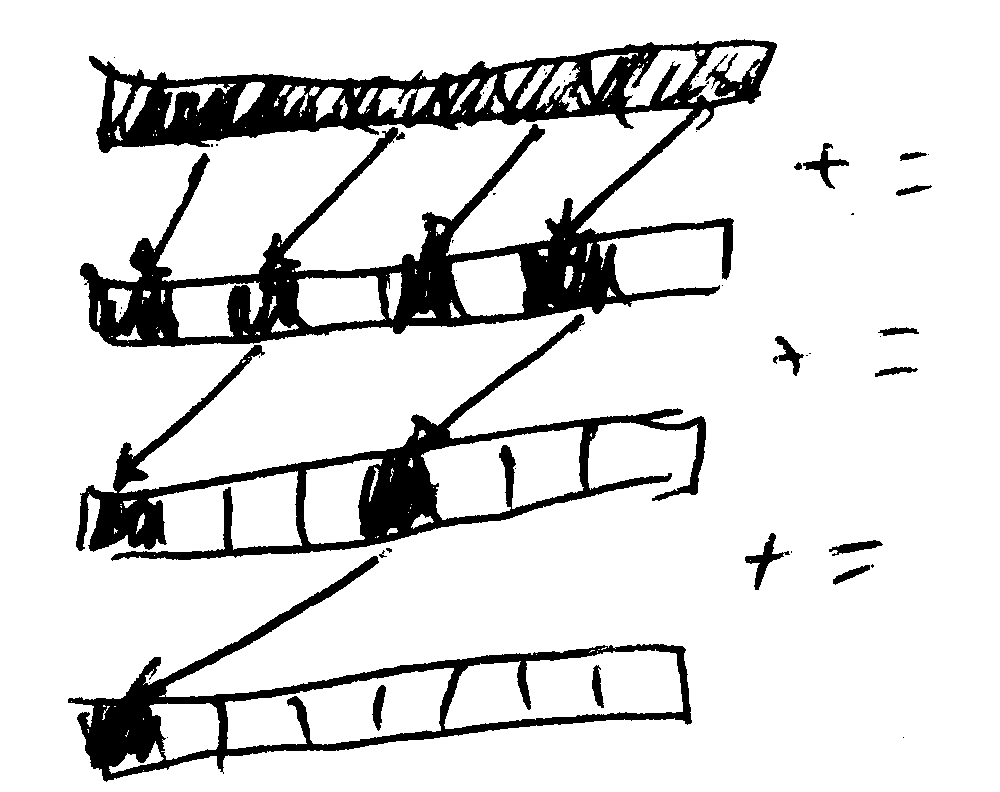
\includegraphics[width=5cm]{warp-2c.png}
  \caption{Exemplo de warpSize}
  \label{fig:warp}
\end{figure}

\begin{verbatim}
for com (ints =warSize >> 1; s>0; s >>=1)
\end{verbatim}
(Estudar este for). Está dividindo por dois com o \textit{rigth shift} $>>$.

\textsc{warp shuffle}: forma ainda mais rápida de fazer o segundo for dele. Conferir o que é um \texttt{threadblock}. Mais nos conceitos.

AOS e SOA: Diferenças:
\begin{itemize}
	\item SOA é melhor em shared memory.
	\item AOS é usada em global memory.
\end{itemize}

\textsc{Uso de atomic memory}: Devem ser minimizados. É mais lento quando tem competição. Exemplo:
\begin{verbatim}
__threadFence();
\end{verbatim}

$\rightarrow$ Make sure the value is propagated to all.

Google: \texttt{atomicInc(...)} $\rightarrow$ usar apenas limitadas a 1 ou 2 por threadblocks.\\ 
\textsc{Privatization scheme}: coarser granularity. warps, thread-blocks... Divisão granular. Shared memory é um tipo de "privatização". Off-GPU memory access. 
Vale a pena ter pequenos vários acessos à memória (o termo é zero-copy).

\end{document}
